\documentclass[fancybox]{seminar}

\usepackage{semcolor}
\input{seminar.bug}
\usepackage{pstcol}
\usepackage{pst-grad}
\usepackage{slidesec}
\usepackage{fancybox}
\usepackage{graphicx}


\newenvironment{code}
  {\begin{list}{}{
    \setlength{\rightmargin}{\leftmargin}
    \raggedright
    \setlength{\itemsep}{0pt}
    \setlength{\parsep}{0pt}
    \ttfamily}%
   \item[]}
  {\end{list}}

\newcommand{\heading}[1]{%
  \begin{center}
    \Ovalbox{\large\bf #1}
  \end{center}
  \vspace{1ex minus 1ex}}

\definecolor{Gold}{rgb}{1.,0.84,0.}
\slideframe{scplain}

\begin{document}

\begin{slide}

\heading{What I'm doing}

\begin{itemize}
\item Research into {\em dynamic optimisation}
\item In particular:
  \begin{itemize}
  \item Support features in an instruction set
  \item Profiling strategy
  \item Optimisation strategy
  \end{itemize}
\end{itemize}

\end{slide}


\begin{slide}

\heading{New work}

\begin{itemize}
\item Working ELF toolchain (assembler \& linker)
\item Semi-working C compiler
\item Working 3-stage pipeline simulator
\item Tweaks to instruction set
\item Designed an optimisation strategy
\end{itemize}

\end{slide}


\begin{slide}

\heading{Planned work}

\begin{itemize}
\item Implement optimisation algorithm
\item Create working compiler backends
\item Do some experiments
\item Get some results
\end{itemize}

\end{slide}


\begin{slide}

\heading{Overview of runtime system}

\begin{figure}[h]

\begin{center}
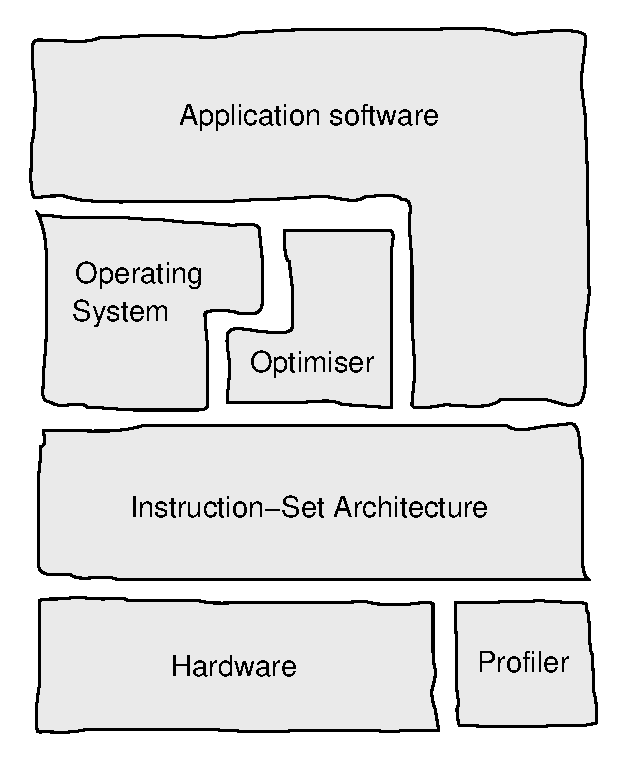
\includegraphics[height=5cm]{runtimeov.ps}
\end{center}

\end{figure}

\end{slide}


\begin{slide}

\heading{Architecture for dynamic optimisation -- DOP}

\begin{itemize}

\item High-level, malleable code layout

\item Simple instruction semantics and encoding

\item ``Hints'' for run-time optimizer in compiled code

\end{itemize}

\end{slide}


\begin{slide}

\heading{Instruction encoding}

\begin{itemize}
\item Handful of instruction formats
  \begin{itemize}
  \item ALU
  \item Single register transfer
  \item Multi-register transfer
  \item Comparison
  \item Flow transfer
  \end{itemize}
\item Lots (64+64) of registers
\item Easy to execute, easy to analyse
\end{itemize}

\end{slide}


\begin{slide}

\heading{Code layout}

\begin{itemize}

\item Instructions are grouped into {\it basic blocks}

\item Code contains \textbf{no} direct branches

\item All control flow is indirected through a table:

\begin{figure}[h]

\begin{center}
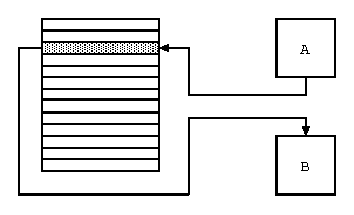
\includegraphics[height=3cm]{indirect-1.eps}
\end{center}

\end{figure}

\end{itemize}

\end{slide}




\begin{slide}

\heading{Rewriting code}

\begin{itemize}

\item Can rewrite code easily

\item B' is an optimised/specialised version of B

\item Also easy to `undo' modifications

\begin{figure}[h]

\begin{center}
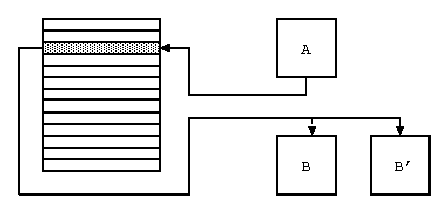
\includegraphics[height=3cm]{indirect-2.eps}
\end{center}

\end{figure}

\end{itemize}

\end{slide}


\begin{slide}

\heading{Rollback property}

\begin{itemize}

\item Program semantics must not change over the following transformation:

\begin{figure}[h]

\begin{center}

\includegraphics{stitch1-4.eps}
\end{center}

\end{figure}

\item We must always be able to replace an optimised block with its predecessor

\end{itemize}

\end{slide}


\begin{slide}

\heading{Unconditional branches}

\begin{itemize}

\item We notice an unconditional branch is executed frequently.

\begin{figure}[h]

\begin{center}
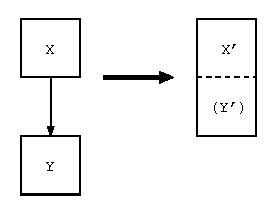
\includegraphics{stitch1-3.eps}
\end{center}

\end{figure}

\item Merge the two blocks together, and perform optimisations, eg:
  \begin{itemize}
  \item Constant propagation
  \item Common subexpression elimination
  \end{itemize}

\end{itemize}

\end{slide}


\begin{slide}

\heading{Conditional branches}

\begin{itemize}

\item If one arm of a conditional branch is executed often:

\begin{figure}[h]

\begin{center}
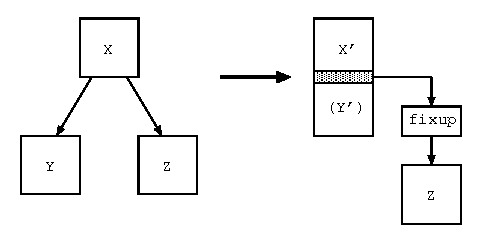
\includegraphics{stitch1-2.eps}
\end{center}

\end{figure}

\item Insert trap in merged block, executed {\it infrequently}

\item Might need fixup code

\end{itemize}

\end{slide}


\begin{slide}

\heading{Function inlining}

\begin{itemize}

\item A function might be inlined incrementally:

\begin{figure}[h]

\begin{center}
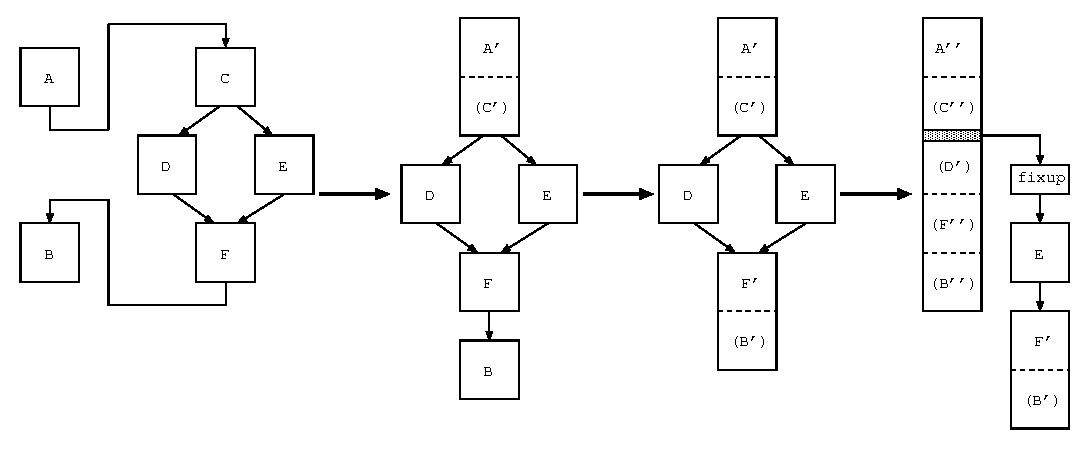
\includegraphics[scale=0.55]{stitch1-5.eps}
\end{center}

\end{figure}


\end{itemize}

\end{slide}


\begin{slide}

\heading{Loop unrolling}

\begin{itemize}

\item If we create/discover a block which conditionally branches to itself:

\begin{figure}[h]

\begin{center}
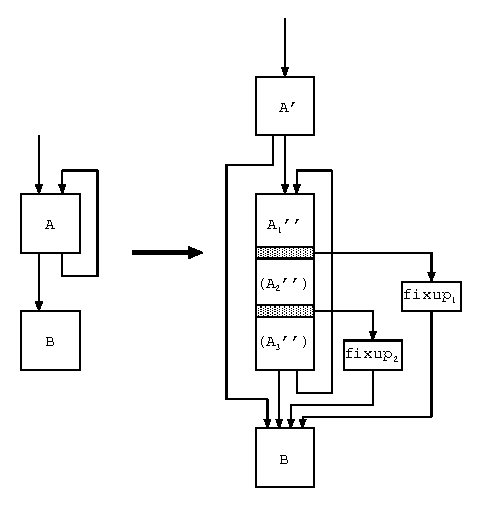
\includegraphics[scale=0.7]{stitch1-6.eps}
\end{center}

\end{figure}

\end{itemize}

\end{slide}


\begin{slide}

\heading{Profiling using transition counters}

\begin{itemize}

\item Lots of counters in an array for profiling

\item Count transitions from one block to another block

\item Hashed by function of both block addresses

\item Reset on collision

\item Trigger optimiser on threshold

\item Victim cache?

\end{itemize}

\end{slide}


\end{document}
